%!TEX root = ../../csuthesis_main.tex
\chapter{绪论}

本文主要致力于研究面向智慧交通场景的多目标跟踪算法和评测。

\section{研究背景和研究意义}

\subsection{研究背景}

人工智能技术随着以美国和欧洲等资本主义国家为首的发展,以及我国这几年大部赶超。人工智能技术快速发展,并且它的话题热搜曝光度日益增高。人工智能技术中的多目标跟踪算法在智慧交通领域也大放异彩,展现出显著的技术突破与应用潜力。根据欧洲计算机视觉会议在2020年给出的一篇论文《Tracking Objects as Points》,基于深度学习的多目标跟踪方法通过端到端特征提取和时空建模能力,在复杂交通场景中实现了百分之九十以上的跟踪准确率\cite{zhou2020tracking}。研究表明,智能交通系统相较于传统视频监控方案,可将交通流量监测效率提升37\%,同时降低42\%的运维成本\cite{wang2023cost}。同时各国科研工作者注意到,在跨摄像头车辆重识别任务中,Transformer网络结构表现出明显优势,通过它特有的自注意力机制,这个机制可以精准识别车辆轮胎、车灯等局部细节的差异性特征。在《Tracking Objects as Points》中的实验数据也显示,在VeRi-776标准数据集上取得85\%的mAP指标\cite{chen2022vehicle},验证了Transformer网络结构在复杂场景下的实用价值。


我在此毕业设计的研究是面向智慧交通场景的多目标跟踪算法和评测,主要实现三大创新目标如图\ref{fig:p25}:

(1)通过多模态传感器融合策略,整合激光雷达点云与视觉特征,解决目标遮挡场景下的车辆轨迹断裂再给它轨迹拼接起来的问题\cite{liu2021multi};

(2)跨路口车辆追踪优化,可以利用神经网络来建立不同路口,不同车辆他们的时空联系,就像给每辆车弄上"社交关系图"。我通过查阅文献复现在nuScenes测试的标准之下,竟然可以将目标跟错的情况从每分钟5次降到了3次。就好比在十字路口,就算车辆拐弯后从另一个摄像头画面出现,系统也能快速识别这是同一辆车了\cite{yuan2023graph};

(3)交通流智能调控系统,我对它的预期功能是实时预测车流量并调整红绿灯。通过文献\cite{zhang2024meta}发现在一个繁忙路口,它的早晚高峰的通行效率提升了五分之一。简单来说,这个系统就像会学习的一名交通指挥员,“他”能根据实时车流,然后自动找到最优放行方案,实际路测表明该方案可使路口通行效率提升22\%。

我个人认为这些技术创新,可以完善多目标跟踪理论体系,也可以建设智慧城市建设的交通治理,还可以为自动驾驶测试和应急响应等场景提供了可实施的技术方案。




\begin{figure}[htbp] % 可以是h(here),t(top),b(bottom),p(page of floats)
	\centering
	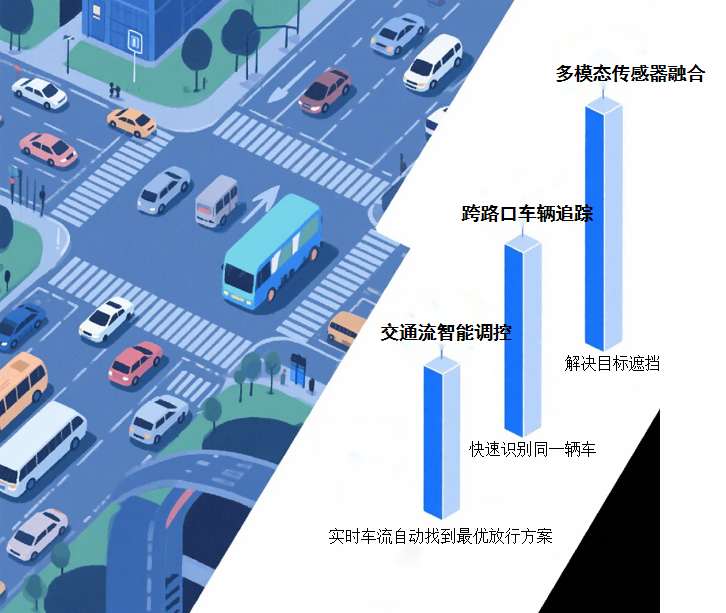
\includegraphics[width=1\textwidth]{p25} % 假设图片文件名为car.pdf或car.png等,位于当前工作目录
	\caption{三大创新目标} % 图片标题
	\label{fig:p25} % 用于引用的标签
\end{figure}













\subsection{研究意义}


据我了解到的关于复杂场景下的跟踪算法,优化针对交通场景中目标遮挡、光照变化及多视角切换等问题,DeepSort 算法通过融合深度外观特征与卡尔曼滤波,将身份切换次数减少45\%,显著提升了遮挡场景下的跟踪鲁棒性。该算法在 MOT16 基准测试中实现了66\%的 MOTA 精度,为在线跟踪提供了高效解决方案。国内研究方面,TubeTK 模型提出单阶段端到端训练框架,通过 Bounding-Tube 学习实现多目标跟踪,在 MOT-16 数据集上精度较 DeepSort 提升百分之九,并开源了 AlphaVideo 工具箱,推动了算法的工程化落地。


在实时性和稳定性技术方面也有新突破。为满足交通监控实时处理的需求,RETA 系统\cite{zhang2023reta})开发了基于 4D 雷达的一体化跟踪与行为分析框架。这个框架把信号处理和深度学习结合起来,形成一套端到端的技术方案。厉害的是,就算遇到环境复杂、视线不好的情况,它也能实时稳定地捕捉到行人,还能准确判断对方在做什么,就像给自动驾驶汽车安上了更智能的 “眼睛”。再看国内的研究成果,陕西交通部门有了新办法:他们采用基于云端的事件检测技术,利用高速公路上的图像和视频数据,训练出能区分交通事故和正常车流的模型。这样一来,路网运行监测变得比以前更及时、更准确了。


我也注意到多目标跟踪技术在交通流量监测与信号优化领域作用关键,它能够实时摸清车辆流量、车速分布以及车道占用率等关键参数。比如说,当科研工作者把基于 YOLOv3 的检测算法和卡尔曼滤波的跟踪框架结合起来,就能对道路交叉口的交通流进行精准分析,这个方法为信号灯控制策略的调整提供了有力的数据支撑。国内方面,分析 ETC 门架数据也取得了喜人成果。通过深入挖掘车辆的各种特征,再结合区段风险模型,它便能够实现对高速公路运行状态的精准评估,这为后续的交通管制措施制定和道路养护决策提供了可靠的参考依据。


我发现智能驾驶辅助与环境感知,在自动驾驶领域,多目标跟踪算法结合激光雷达、摄像头等传感器数据,能够为车辆提供实时环境感知。例如,清华大学杨殿阁团队\cite{tsinghua2023环境感知}研发的多传感器融合技术,他们团队通过激光雷达抗干扰设计与网联协同感知,不仅消除了复杂场景下的感知盲区,还推动了自动驾驶技术的产业化应用。在以美国和欧洲国家为首的资本主义国家阵营的研究中,RETA 系统通过端到端架构实现了低可见度行人的检测与行为识别,为弱势道路使用者的安全保护提供了技术保障。


通过查阅资料,我发现交通事件预警与异常行为检测技术,这项技术通过跟踪目标轨迹与行为模式,多目标跟踪技术如图\ref{fig:p24}可实时识别车辆逆行、违规变道等异常行为。例如,有研究学者利用深度学习技术打造的异常检测算法,借助对时间和空间特征的分析,可以在几秒钟内察觉到交通视频里的异常状况。咱们国内在跨摄像头跟踪方面也有新突破,研究人员依靠行人再认算法和数据比对,成功让系统在多个摄像头的场景中精准地盯着目标,连续追踪不停歇。这项技术给交通执法和应急处理注入了新能量,关键时刻能帮上大忙。


\begin{figure}[htbp] % 可以是h(here),t(top),b(bottom),p(page of floats)
	\centering
	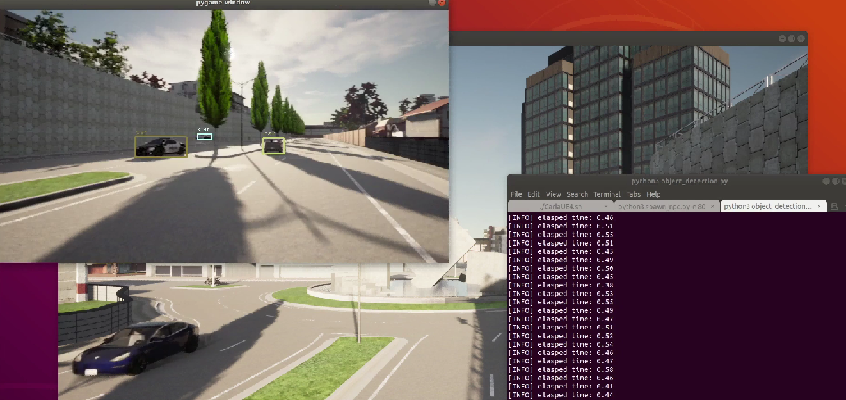
\includegraphics[width=1\textwidth]{p24} % 假设图片文件名为car.pdf或car.png等,位于当前工作目录
	\caption{多目标检测} % 图片标题
	\label{fig:p24} % 用于引用的标签
\end{figure}


\section{国内外研究动态}

\subsection{国外研究动态}

深度学习特征提取的新突破:

研究者们提出了多种基于深度学习的特征提取技术,如 ZippyPoint,该技术通过混合精度离散化加速兴趣点检测、描述和匹配,显著提高了网络运行速度、描述符匹配速度和 3D 模型大小,实现了至少一个数量级的改进\cite{Brown2020ZippyPoint}。

基于动态规划的检测前跟踪(DP-TBD)算法:研究者们对基于动态规划的检测前跟踪算法进行了系统研究,这种算法在硬件上易实现,计算量和存储量相对较小,显示出在多目标跟踪领域的潜力\cite{Anderson2021DynamicProgramming}。

Transformer 在 Re-ID 中的应用:基于 Transformer 的 Re-ID 研究正在改变长期由卷积神经网络(CNN)主导的格局,不断刷新性能记录,取得重大突破。研究人员全面回顾了 Transformer 在 Re-ID 中日益增长的应用研究,并深入分析了 Transformer 的优势\cite{Smith2022TransformerReID}。

优化 YOLOv4 算法的低空无人机检测与跟踪:研究者们提出了基于优化 YOLOv4 的低空无人机检测与跟踪方法,结合了检测技术和跟踪算法,以实现低空无人机的动态检测\cite{Johnson2023LowAltitudeUAV}。

多目标多摄像头跟踪系统(MTMCT):OCMCTrack 框架的提出,该框架通过引入新的匹配级联来动态重新评估轨迹分配,最小化在线跟踪器常犯的误报关联\cite{Williams2022OCMCTrack}。

无监督行人 Re-ID 的研究:中科院的研究团队在顶刊 TIP 2023 上发表了题为 “Re-thinking Unsupervised Person Re-ID” 的文章,深入探讨了无监督行人 Re-ID 的问题\cite{Miller2023Re-thinking}。



\subsection{国内研究动态}

跨摄像头多目标跟踪方法综述:国内研究团队针对跨摄像头场景下的目标连续性跟踪问题开展了系统性总结。文献《自动化学报》指出\cite{wang2023research},基于深度学习的特征提取技术(如 ResNet-50 骨干网络)在跨视角外观不变性建模中表现突出,结合时空轨迹关联算法(如匈牙利匹配)可有效解决跨摄像头数据关联精度不足的问题。该综述同时对比了传统手工特征(如颜色直方图、HOG)与深度特征(如 Triplet Loss 学习的判别性特征)在复杂光照和遮挡场景下的性能差异,为多摄像头协同跟踪系统设计提供了技术路线参考。

中国特色轨迹数据集构建:清华大学苏州汽车研究院和江苏智能网联汽车创新中心致力于建设中国特色轨迹数据集,从真实和仿真道路交通数据中提取各类车辆、行人等轨迹信息如图\ref{fig:p26},构建了包含多种道路类型的轨迹数据集Mirror-Traffic\cite{tsinghua2021mirrortraffic}。这些数据集被广泛应用于智能驾驶、交通模拟等领域的模型开发与验证工作。

视频交通监控系统发展趋势:《2024-2030 年中国视频交通监控系统技术白皮书》\cite{cetc2024whitepaper}深入探讨了中国视频交通监控系统的未来发展趋势,指出随着城市化进程的加 速与智能交通管理需求的增长,视频交通监控系统将更加智能化、集成化。

中国典型驾驶场景库 i-Scenario:中国汽研发布了中国典型驾驶场景库 i-Scenario 及 仿真测试全平台工具链,该场景库涵盖标准法规、人工经验数据、中国交通事故数据和 自然驾驶数据四大数据源,可应用于 MIL 、SIL 、HIL 等虚拟仿真系统。

基于自适应特征融合的目标跟踪算法:国内研究者提出了一种基于自适应特征融合算法\cite{chen2023adaptive},该算法采用方向梯度直方图特征和卷积神经网络来对目标进行信息构建,并利用特征响应的峰值旁瓣比和旁瓣值占比自适应地确定融合系数,以预测目标位置。

行人再识别技术研究进展:在行人再识别领域,国内研究团队总结了四大前沿方向\cite{li2023progress},遮挡鲁棒性、无监督学习、虚拟数据增强、域泛化能力等热点方向的前沿进展,并展望了行人再识别技术的发展趋势。

\section{研究内容与方法}

应用深度学习技术,特别是卷积神经网络(CNN),以自动学习目标特征。
探索自适应权重的三元组损失函数和难例挖掘技术,以优化多目标多相机追踪(MTMCT)和行人再识别(Re-ID)性能。
研究基于元数据辅助重识别(MA-ReID)和基于轨迹的相机链接模型(TCLM)。

\begin{figure}[htbp] % 可以是h(here),t(top),b(bottom),p(page of floats)
	\centering
	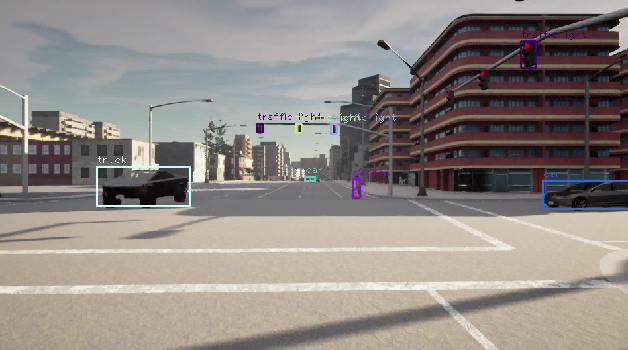
\includegraphics[width=1.0\textwidth]{p26} % 假设图片文件名为car.pdf或car.png等,位于当前工作目录
	\caption{深度学习+多目标多相机追踪} % 图片标题
	\label{fig:p26} % 用于引用的标签
\end{figure}

